\section{Radio Propagation}

\subsection{Free Space}

\begin{tabular}{|l|c|}
	\hline
	Power density                       &                          $ p(d) = \frac{P_t}{4 \pi d^2}$                           \\ \hline
	Received Power                      &              $P_r = p(d) \cdot A_e = \frac{P_t \cdot A_e}{4 \pi d^2}$              \\ \hline
	Antenna Gain [Linear]                        &        $G = \frac{4 \pi \cdot A_e}{\lambda^2} \qquad \lambda = \frac{c}{f}$        \\
	                                    & $\theta_1 \cdot \theta_2 \cdot G \cong 4 \pi \qquad \theta^2 \cdot G \cong 4 \pi $ \\ \hline
	Equivalent Isotropic Radiated Power &                               $EIRP = P_t \cdot G_t$                               \\ \hline
	Rx Power                            &   $P_r(d) = \frac{P_t \cdot G_t \cdot G_r \cdot \lambda^2}{(4\pi)^2 \cdot d^2}$    \\ 
	                                    & $P_r[dBm] = P_t[dBm] + G_t[dBi] + G_r[dBi] - PL_{path}[dB]$ \\ \hline
	Path Loss (Free Space) 				& $PL_{path}[db] = 10\cdot log_{10}((\frac{4\pi d}{\lambda})^2) = 10\cdot log_{10}((\frac{4\pi d\cdot f}{c})^2)$  \\ 
	                                    & $PL_{path}[db] = 32.4\;dB + 20 \cdot log_{10}(f[MHz]) + 20 \cdot log_{10}(d[km])$ \\
										& $D_{max}[m] \leq \sqrt{10^{\frac{PL_{path}[db]}{10}}}\cdot \frac{c}{4\pi f}$ 		\\ \hline
\end{tabular} 

\subsection{Path Loss Model 'Exponent n'}

\begin{equation}
	PL_{path}(d) = \underbrace{PL_{fs}(d_0)}_{\textbf{Free space Loss @ $d_0$}} + 10 \cdot n \cdot log_{10}(\frac{d [m]}{d_0 [m]})
\end{equation}

\begin{equation}
	PL_{fs}(d_0) = 10\cdot log_{10}((\frac{4\pi d_0}{\lambda})^2)
\end{equation}

\begin{table}[!htp]
\begin{subtable}[c]{0.6\textwidth}
	\begin{tabular}{|l|c|}
	\hline \textbf{Enviroment} & \textbf{Path Loss Exponent n} \\ \hline
		\hline Free Space & 2 \\ 
		\hline Urban area cellular radio &  2.7 to 3.5\\ 
		\hline Shadowed urban cellular radio &  3 to 5\\ 
		\hline In Building line-of-sight & 1.6 to 1.8 \\ 
		\hline  Obstruct in building& 4 to 6 \\ 
		\hline Obstruct in factories & 2 to 3 \\ 
		\hline 
	\end{tabular}
\end{subtable}
\begin{subtable}[c]{0.4\textwidth}
	\begin{tabular}{|l|c|}
	\hline \textbf{Enviroment} &  \textbf{Distance $d_0$ }\\ \hline
	\hline Indoor Office & 1 m \\ 
	\hline Indoor Factory & 10 m \\ 
	\hline Outdoor Urban & 100 m \\ 
	\hline Outdoor Rural & 1000 m \\ 
	\hline 
	\end{tabular}
\end{subtable}
\end{table}

\subsection{Path Loss Model 'Empirical Model' (Okumura Hata)}
\subsubsection{Hata Model}
The Hata model for mobile radio is valid under the following constraints:\\ \\
\begin{tabular}{|l|c|}
\hline \textbf{Parameter} & \textbf{Value} \\ \hline
\hline Frequency $f$ & 1500 MHz to 2500 MHz \\ 
\hline Tx height $h_t$ & 30 m to 200 m \\ 
\hline Rx height $h_r$ & 1m to 10 m \\ 
\hline Distance $d$ & 1 km to 20 km \\ 
\hline 
\end{tabular} \\ \\

General Form:
\begin{equation}
	PL_{50}[dB] = A + 10 \cdot n \cdot log_{10}(d[km])
\end{equation}

Median value of the attenuation:
\begin{equation}
	PL_{50}[dB] = \underbrace{ 46.3  33.9 \cdot log(f_c [MHz]) - 13.82 \cot log_{10}(h_t [m]) -a(h_r  [m])}_{A} +  \underbrace{(44.9 -6.55 \cdot log_{10}(h_t [m]))}_{10 \cdot n} \cdot log_{10}(d [km]))
\end{equation}
\begin{equation}
	a(h_r) = (1.1 \cdot log_{10}(f_c) - 0.7) \cdot h_r- (1.56 \cdot log_{f_c} - 0.8)
\end{equation}

\textbf{If height of the tx antenna $h_t = 30\;m$ then is $n=3.5$. The result rate is then $\frac{35\;dB}{Dekade}$}


\subsubsection{Okumura Hata Model}
The Okumura Hata model for mobile radio is valid under the following constraints:\\ \\
\begin{tabular}{|l|c|}
\hline \textbf{Parameter} & \textbf{Value} \\ \hline
\hline Frequency $f$ & 150 MHz to 1500 MHz \\ 
\hline Tx height $h_t$ & 30 m to 200 m \\ 
\hline Rx height $h_r$ & 1m to 10 m \\ 
\hline Distance $d$ & 1 km to 20 km \\ 
\hline Distance $d$ & 1 km to 20 km \\ 
\hline 
\end{tabular} \\ \\

Urban Path Loss:
\begin{equation}
	PL_{50,Urban}[dB] =  69.55 + 26.16 \cdot log_{10}(f [MHz])- 13.82 \cdot log_{10}(h_t [m]) - C+ (44.9 -6.55 \cdot log_{10}(h_t[m])) \cdot log_{10}(d[km]))
\end{equation}

Correction factor C:\\ \\
\begin{tabular}{ll}
medium/small cities: & $C = (1.1 \cdot log_{10}(f [MHz])-0.7) \cdot h_r -1.56 \cdot log_{10}(f [MHz]) + 0.8 \quad \text{ ~ } 0 \text{ if } h_r = 1.5m$ \\ 
suburban: & $C = 2 \cdot (log_{10}(\frac{f[MHz]}{28}))^2 + 5.4$ \\ 
\end{tabular} 

\subsection{Link Budget}
Received Power:
\begin{equation}
	P_r [dBm] = \underbrace{P_t [dBm] - L_t [dBm] + G_t[dBi]}_{ \text{EIRP [dB]} } - PL_{path}[dB] + G_r[dBi] -L_r[dB]
\end{equation}

\begin{tabular}{ll}
\textbf{Parameter} & \textbf{acceptation} \\ \hline
$L_t$ & wire loss of tx \\ 
$L_r$ & wire loss of rx \\ 
$EIRP$ & often limited by regulation \\ 
\end{tabular} \\ \\

Minimum required Rx Power
\begin{equation}
	P_r [dBm] \geq \underbrace{-174[dBm]}_{ \text{noise floor} } + 10 \cdot log_{10}(\underbrace{B [Hz]}_{\text{bandwidth} }) + 
	\underbrace{F_{tot}[dB]}_{ \text{Rx noise figure} } + SNR_{min} + Margin_{ \text{Fading} }
\end{equation}

\subsection{Das zelluläre Konzept \formelbuch{235}}
	\begin{minipage}{12cm}
		Gesamte Fläche bspw. eines Landes wird in \textbf{sechseckige Flächen} - sogenannte \textbf{Zellen} - aufgeteilt. 
		Eine \textbf{Gruppe} von Zellen - ein sog. \textbf{Cluster} - enthält nur Zellen mit unterschiedlichen Frequenzen.
		Die Anzahl Zellen pro Cluster $N$ ist durch folgende Formel beschränkt:
		\begin{center}
	        $ N=i^2+j^2+ij = \left\{1,3,4,7,9,12,13,16,19,\ldots\right\}, \quad \text{mit } i,j \in
	        \{0,1,2,3,\ldots \} $ \\ Frequenzwiederholabstand $ D = \sqrt{3N} R = (6\cdot 10^(\frac{C/I[dB]}{10}))^{1/4} R$ \\ Normierter Frequenzwiederholabstand $q = \frac{D}{R} =
	        \sqrt{3N}$ \\ Clustergrösse $N \geq \frac{q^2}{3}$
        \end{center}
	\end{minipage}
	\begin{minipage}{8cm}
	    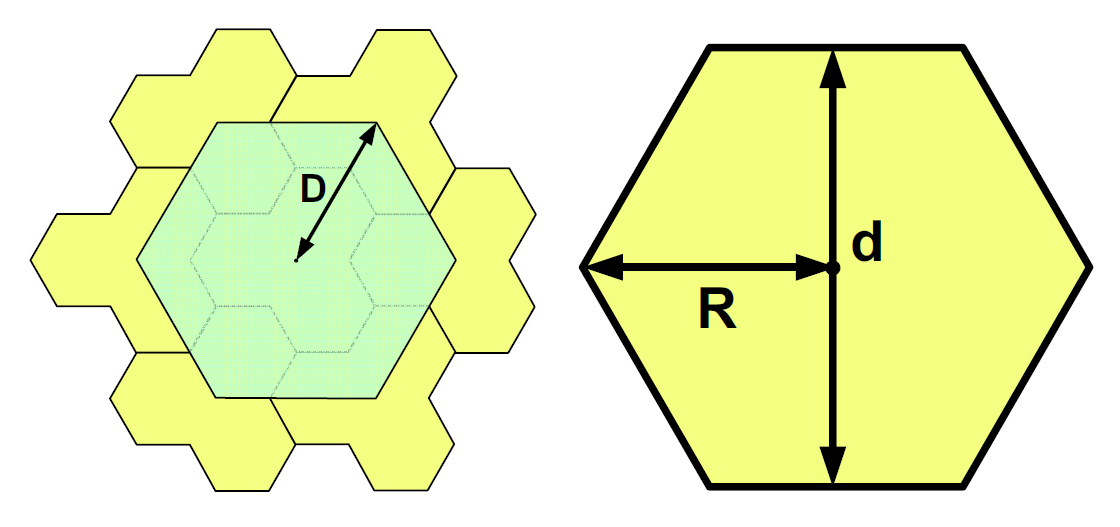
\includegraphics[width=7cm]{./bilder/systems-cluster.png}
	\end{minipage}

\subsubsection{Cochannel Interference $C/I$ \formelbuch{238}}
    \begin{minipage}{12.5cm}
        Interferenz von nächster Zelle mit gleicher Frequenz wird als Cochannel Interferenz $C/I$ angegeben.
        $$ C/I_{\text{lin}} = \frac{r^{-4}}{6d^{-4}} = \frac32 N^2 \qquad \Rightarrow \qquad 
        C/I_{\text{dB}} = 1.76 + 20 \logd N $$
        \begin{center}
            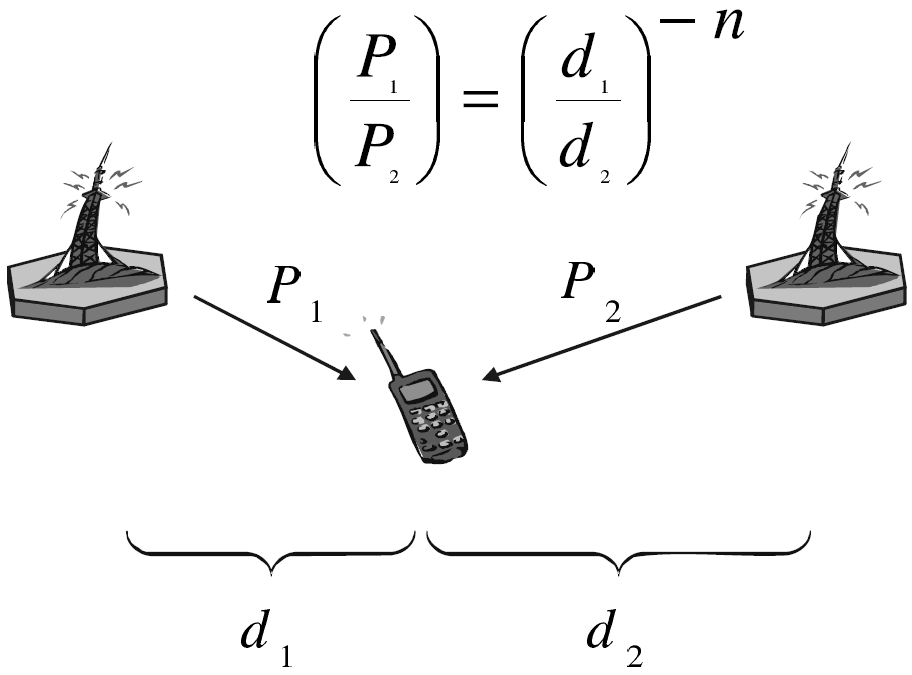
\includegraphics[width=3cm]{./bilder/systems-ci.png}                
        \end{center}
    \end{minipage}
    \begin{minipage}{6.5cm}
        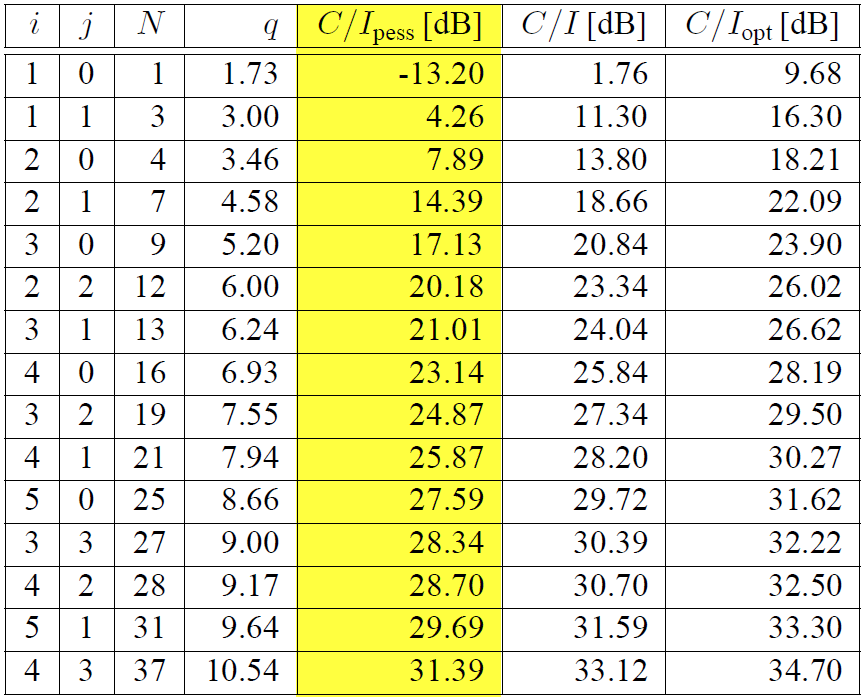
\includegraphics[width=6.5cm]{./bilder/systems-gsm-CItable.png}    
    \end{minipage}

\subsubsection{Sektorisierung \formelbuch{239}}
	Durch Sektorisierung wird die $C/I$ wird um \textbf{Faktor 3 gesteigtert}. Die Antenne wird im Zentrum der Zelle
	aufgestellt und deckt 1/3 der Zelle ab. \textcolor{green}{Vorteile:} $C/I$ verbessert $\Rightarrow$ Clustergrösse kann reduziert werden;
	\textcolor{red}{Nachteile:} Zusätzlicher Hardwareaufwand (Richtantennen, \ldots), Mehr Frequenzen benötigt, Mehr Signalisierung wegen häufigerem Kanalwechsel.

\subsection{Bündelung / Erlang (Trunking)  \formelbuch{240}}
    \begin{minipage}{12cm}
    Nebst der Einteilung in verschiedene Kanäle (FDMA) werden die Benutzer in Zeitschlitze (TDMA) gebündelt,
    um eine grössere Kapazität zu erreichen. \\
    Der Datenverkehr in Mobilfunknetzen wird in \textbf{Erlang} gemessen:
    \begin{liste}
        \item 1 Erlang $\Rightarrow$ 1 Benutzer telefoniert 100\% der Zeit
        \item 2 mE $\Rightarrow$ 1 Benutzer telefoniert 0.2 \% der Zeit
    \end{liste} 
    \vspace{0.2cm}
    Die Wahrscheinlichkeit, dass ein Benutzer blockiert wird und das Telefonat nicht ausführen kann ist gegeben durch
    \text{P(blocking)}:        
        \begin{minipage}{6cm}
            $$   \text{P(blocking)} = \frac{\frac{A^C}{C!}}{\sum_{k=0}^C\frac{A^k}{k!}} , $$            
        \end{minipage}
        \begin{minipage}{4.5cm}
            $A$: Traffic intensity, $[A] = E$ \\        
            $C$: Anzahl Kanäle, $[C] = 1$           
        \end{minipage}       
    Die nebenstehende Grafik zeigt die Blockierungswahrscheinlickeit abhängig von der Traffic Intensity und der Anzahl Kanäle. 
    \end{minipage}
    \begin{minipage}{0.3cm}
        \quad
    \end{minipage}
    \begin{minipage}{7cm}    
        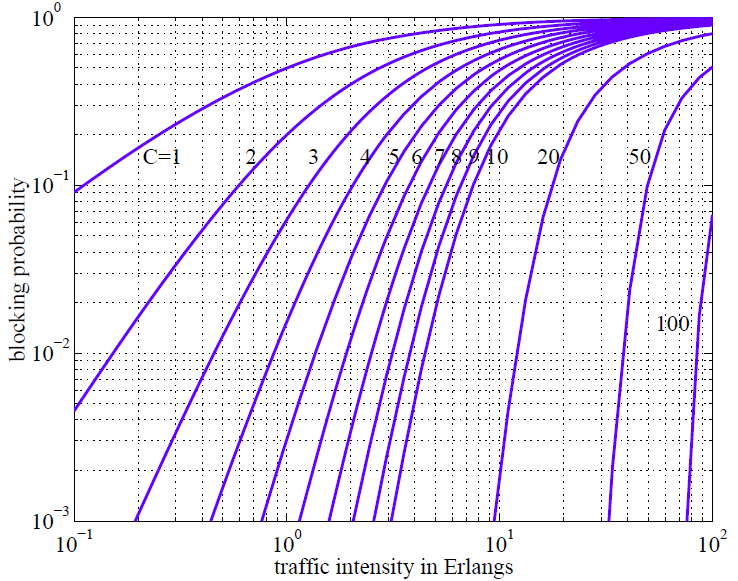
\includegraphics[width=7cm]{./bilder/systems-erlangB-graph.png}
    \end{minipage}